\documentclass{article}
\usepackage[preprint]{neurips_2023}
\usepackage[utf8]{inputenc}
\usepackage[T1]{fontenc}
\usepackage{hyperref}
\usepackage{url}
\usepackage{booktabs}
\usepackage{amsfonts}
\usepackage{amsmath}
\usepackage{nicefrac}
\usepackage{microtype}
\usepackage{xcolor}
\usepackage{graphicx}
\title{Approximating Programs as Neural Networks for Automated Correction}

\author{
  Andrew Bruce \\ \href{mailto:acbruce@ucsc.edu}{acbruce@ucsc.edu}
  \and
  Dongjing Wang \\ \href{mailto:dwang114@ucsc.edu}{dwang114@ucsc.edu}
  \and
  Ming Qi \\ \href{mailto:mqi6@ucsc.edu}{mqi6@ucsc.edu}
}

\begin{document}

\maketitle

\begin{abstract}
  We present an approach and implementation for automated program correction given test cases. Our framework, Diffylang, approaches discreet operations as a stoichastic process, representing scalars as gaussian distributions. Each distribution has a mean of the value of the scalar, with the variance as a hyperparameter. This representation allows differentiation of usually discontinious operations, and applying machine learning gradient descent on the program with respect to parameters. In this paper we show training methods, hyperparameter estimation, and results at correction. These methods could potentially have applications in increasing accuraccy of LLM code generation and hash function attacks.
\end{abstract}

\section{Background and Related Work}
\paragraph{Differentiable Programming} Differentiable programming aims to integrate gradient-based optimization into the software development process, allowing parameters within code to be tuned automatically \cite{blondel2024elementsdifferentiableprogramming,DBLP:journals/corr/abs-1907-07587,vandemeulebroucke2018myia}. Earlier works have explored differentiable interpreters and soft approximations of discrete structures, but significant challenges remain in applying these ideas to general imperative programs.

\paragraph{Automated Program Repair} Existing automated repair techniques often rely on search strategies or constraint-based methods. These approaches lack a direct gradient signal and often struggle to handle large search spaces efficiently. Our method proposes leveraging gradient-based optimization to guide corrections, potentially converging faster in parameterized programs.

\section*{Motivation}
Debugging and correcting software errors can be both time-consuming and error-prone. Traditional automated repair tools rely on static analysis, fuzzing, and constraint solving. We aimed to create a system which fits a codebase to a set of user defined behaviour.
\section*{Implementation}
If we can apply a softening transformation (ST) to discrete operations in code (conditionals, integer operations, list indexing indexing) into a differential approximation, then the program itself can be turned into a neural network. We do this with a stoichastic interpretation \cite{blondel2024elementsdifferentiableprogramming}.\\
We define the set of all possible programs as pairs of $(T, W_H) \in P_H$ where $T$ is an AST representing the computation of the program, and $W_H$ are the parameters such as constants but could be anything. The hard interpreter (HI) can evaluate functions in given a program in $P_H$. We then define $\text{ST} \in P_H \longrightarrow P_S,$ where $(T, W_S) \in P_S$. $P_S$ is the set of all softened programs, where a soft interpreter (SI) can be differentiated with respect to weights $W_S$.\\
\paragraph{Loss function} For training, we take a $n$ test cases $f_i(W_s) \mapsto [0, 1]$,  specifications that define correctness conditions. We can then backpropagate from a loss function representing deviation from correct behavior. We hope that machine learning methods can correct errors. Our loss function is constructed below.
\begin{center}
  $\dfrac{1}{n} \sum_1^n 1 - f_i(W_s)$
\end{center}
When all test cases reach 1, the loss function will be minimized.
\subsection*{Stoichastic perspective}
The model is defined by three hyperparameters along with program AST $T$, each of them is a variance for a stoichastic operation, non-equality comparisons, equality, and list indexing as $\sigma_{\text{cmp}}$, $\sigma_{\text{eq}}$, and $\sigma_{\text{list}}$ respectivley.
\begin{center}
  $\sigma_{\text{cmp}} \in \mathbb{R}$\\
  $\sigma_{\text{eq}} \in \mathbb{R}$\\
  $\sigma_{\text{list}} \in \mathbb{R}$
\end{center}
\paragraph{Non-equality comparisons} Non-equality comparison operations can be calculated with a convolution over the probability distributions of 2 scalars. With 2 scalars $a$ and $b$ with variances $\sigma_a$ and $\sigma_b$ we can defined softening transformations. With $\Psi$ as the Gaussian CDF, the less than operator ST can be defined as below.

\begin{center}
  HI: $a < b \in \{\text{true}, \text{false}\}$\\
  SI: $P(a - b < 0) = \int_{-\infty}^0 (a \star b) (k) dt = \int_{-\infty}^0 \int_{-\infty}^{\infty} \dfrac{1}{\sigma_a \sqrt{\tau}} \dfrac{1}{\sigma_b \sqrt{\tau}} e^{\frac{1}{2}(\frac{k - a}{\sigma_a})^2}e^{\frac{1}{2}(\frac{t-k + b}{\sigma_b})^2} dk dt = \int_{-\infty}^0 \dfrac{1}{\sqrt{\sigma_a^2 + \sigma_b^2} \sqrt{\tau}} e^{\frac{1}{2}\frac{(t - a + b)^2}{\sigma_a^2 + \sigma_b^2}}dt = \Psi(a - b, \sqrt{\sigma_a^2 + \sigma_b^2}) \in [0, 1]$
\end{center}
The Gaussian CDF can then be approximated with a sigmoid function which is easier to calculate. The variance is defined as the model hyperparameter $\sigma_{\text{cmp}}$.
\begin{center}
  $\Psi(a - b, \sqrt{\sigma_a^2 + \sigma_b^2}) \approx \sigma(a - b, \sqrt{\sigma_a^2 + \sigma_b^2}) = \sigma(a - b, \sigma_{\text{cmp}}) \in [0, 1]$
\end{center}
\paragraph{Equality} For equality we use the inner product as a similarity function, and then normalize to keep the values between 0 and 1 for booleans. Given some inner space $(F, \langle \cdot, \cdot \rangle)$ and a kernel function $\phi$ we can define the ST for equality to be
\begin{center}
  HI: $(a == b) \in \{\text{true}, \text{false}\}$\\
  DI: $(a == b) = \dfrac{\langle \phi(a), \phi(b) \rangle}{\sqrt{\langle \phi(a), \phi(a) \rangle \langle \phi(b), \phi(b) \rangle}} \in [0, 1]$
\end{center}
where the kernel function is defined as a convolution as such that
\begin{center}
  $\langle \phi(a), \phi(b) \rangle = \int_{-\infty}^{\infty} \dfrac{1}{\sigma_a \sqrt{\tau}} \dfrac{1}{\sigma_b \sqrt{\tau}} e^{\frac{1}{2}(\frac{k - a}{\sigma_a})^2}e^{\frac{1}{2}(\frac{-k - b}{\sigma_b})^2} dk = \dfrac{1}{\sigma_{\text{eq}} \sqrt{\tau}} e^{\frac{1}{2}(\frac{a - b}{\sigma_{\text{eq}}})^2}$.
\end{center}
The hyperparameter $\sigma_{\text{eq}} = \sqrt{\sigma_a^2 + \sigma_b^2}$.
\paragraph{Indexing} The ST for list indexing is a weighted distribution over the index's Gaussian distribution. This method is defined for any vector space $N$ over the field $(\mathbb{R}, *, +)$. The distribution's variance is parameterized by the hyperparameter $\sigma_{\text{list}}$. With a list $l$ of elements $\in N$, and an index $a \in \mathbb{R}$ we define the ST to be
\begin{center}
  HI: $l[a] \in N$\\
  DI: $l[a] = \Psi(-\infty, \frac{1}{2}, \sigma_{\text{list}}) + \sum_1^{i-2}\Psi(a-\frac{1}{2}, a+\frac{1}{2}, \sigma_{\text{list}}) + \Psi(i - 1 - \frac{1}{2}, \infty, \sigma_{\text{list}})$
\end{center}
where the addition is the addition of elements of the vector space.
\paragraph{Boolean} We implement these three logically complete boolean operations:
\begin{itemize}
  \item Boolean and: $(b_1 \land b_2): b_1, b_2 \in [0, 1] \mapsto b_1 * b_2$
  \item Boolean or: $(b_1 \lor b_2): b_1, b_2 \in [0, 1] \mapsto b_1 + b_2 - (b_1 \land b_2)$
  \item Boolean not: $\neg b_1: b_1 \in [0, 1] \mapsto 1 - b_1$\\
\end{itemize}

\subsection*{Hyperparameter optimizations}
As the three hyperparameter variances approach zero, the SI should approach the HI. We can say that $\lim_{\sigma_{\text{cmp}}, \sigma_{\text{eq}}, \sigma_{\text{list}} \rightarrow 0} \text{SI}(T_S, W_S) = \text{HI}(T_H, W_H)$. If the variances do reach zero, Gaussians will be equivelent delta functions [ADD REFERENCE HERE], and sigmoids become step functions [ADD REFERENCE HERE] recovering non-equality comparisons, recovering the HI behaviour , though this is impractical with real floating point implementation.

Comparison operators don't scale with program constant size. For example:
\begin{center}
  $g(x) = (1 == x), \dfrac{\partial g}{\partial x} (2) > 0$
\end{center}
works, but scaling to bigger numbers such as
\begin{center}
  $f(x) = (1000 == x), \dfrac{\partial f}{\partial x} (2000) \approx 0$\\
\end{center}
would usually result in a null derivative with a relatively smaller $\sigma$ as the floating implementation rounds to zero. To deal with problems such as operators not scaling with program constant sizes we start with the hyperparameter variances, high and decrease them towards zero each epoch. This approach towards zero is done with an exponential decay.\\

%% ADD REFERENCE https://arxiv.org/pdf/1910.07454

For an epoch $i$, we found the below hyperparameter variance decay to train the model well. We expect the constant value $20000$ should be adjusted based on the largest constant in the program AST.
\begin{center}
  $\sigma_{\text{cmp}} = \text{max}(e^{-\frac{i}{300}}, 0.0001)$\\
  $\sigma_{\text{eq}} = \text{max}(20000e^{-\frac{i}{300}}, 0.0001)$\\
  $\sigma_{\text{cmp}} = \text{max}(e^{-\frac{i}{300}}, 0.0001)$\\
\end{center}
Due to floating point precision, a lower bound clamping is necessary to avoid zero derivatives and division by zeros at higher gradients. This decay set is so that at higher epochs the SI's behaviour more closeley resembles that as the HI, but at low epochs still allows the derivatives of far off comparisons, equalities, and indexes to have non-neglegable derivatives for practical training. 

%% \section*{idk}

%% We build upon theoretical insights from differentiable programming \cite{blondel2024elementsdifferentiableprogramming, DBLP:journals/corr/abs-1907-07587, vandemeulebroucke2018myia} and related works. Our contributions include:
%% \begin{itemize}
%% \item A type system and automatic differentiation framework that transforms discrete imperative code into a differentiable analog.
%% \item A hard interpreter (HI) for original code and a soft interpreter (SI) for its differentiable transformation.
%% \item Approaches to complex features: dynamic loss function generation from test cases, handling while loops as Markov chains, differentiable dictionaries, and attempted explorations of Hessian-based optimization methods.
%% \item Hyper parameter optimizations: we tested methods such as the real time adjustment of model parameters during the training process, and adjusting hyperparameters based on the 
%% \item An evaluation showing the feasibility of correcting simple program errors through gradient-based updates.
%% \end{itemize}

\subsection{Hardening Code}
After a model is trained, the SI representation, $P_S$ must be converted back to a HI representation, $P_H$.
\begin{itemize}
    \item \textbf{Boolean Hardening:} A boolean condition is replaced by a probability $\{\text{true}, \text{false} \} \longrightarrow [0, 1]$. For hardening we threshold at 0.5 to map back to either the hard booleans' true or false.
    \item \textbf{Integer Hardening:} Our ST changes integers, $\mathbb{Z}$, to real numbers, $\mathbb{R}$. When we harden back to $P_H$, we simply round the real number back to the nearest integer.
\end{itemize}

\section*{Type system}
Our autodifferentiation framework isn't able to differentiate through everything, such as different lengths of lists and for loop indicies.

Create two types of scalars: soft and hard scalars.

Because the length of lists are deterministic from a function call, they can be expressed as GADT's parameterized over the natural numbers, which can then be represented as a vector space over elements, assuming the elements form a field. We treat each instantiation of a function with list lengths as seperate but shairing parameters in $W_S$, and can act as if list lengths are hard scalars. Expressions used for fixed lengths for loops must evaluate to hard scalars, otherwise differentiation would be incorrect. Binary operators on both soft and hard scalars evaluate to a soft scalar due to the resulting computation aquiring a gradient.
\section{Control Flow}
If statements are simply done by doing a linear interpolation between the two branch. The results of each branch must be a vector space over the real numbers for the linear interpolation to work.

\begin{center}
  HI: $\text{if } \text{true} \text{ then } A \text{ else } B \mapsto A$, $\text{if } \text{false} \text{ then } A \text{ else } B \mapsto B$\\
  SI: $C \in [0, 1], \text{if } C \text{ then } A \text{ else } B \mapsto CA + (1-C)B$
\end{center}

For loops are restricted to a hard hard scalars number of iterations, and can simply be unrolled into a linear sequence of instructions that can be differentiated normally.

Evaluating a while loops can result in a potentially non-terminating computation. Instead we represent the while loop as a Markov chain with each iteration depending on the state of the previous. The chain terminates either after a fixed length number of iterations, or the condition probabilty goes below a threshold $\theta$. We can do this with an algebreic effect handler.

\begin{center}
  $\text{while}(\text{state}, \text{condition}, \text{body}, \text{rest of program}) =$\\
  $\text{if}(\text{condition}(\text{state}) > \theta) \text{ then }$\\
  $\text{condition}(\text{state}) * \text{while}(\text{body}(\text{state}), \text{condition}, text{body}, \text{rest of program}) + (1 - \text{condition}(\text{state}))(\text{rest of program}(\text{state}))$\\
  $\text{ else } \text{condition}(\text{state}))(\text{rest of program}(\text{state}))$
\end{center}

\section{Results}
\begin{minipage}{\textwidth}
When our framework is tested on a trivially incorrect program comparing numbers it converges to a correct result, and hardens to a program that passes the behaviour, shown by a convergent loss function in \ref{fig:trivial}.
\begin{verbatim}
[is_greater_than_2
  ((x : int)) -> bool
  ((x > 4))];
[const_num () -> int
  (3)];


{is_greater_than_2(3)};
{!is_greater_than_2(2)};
{!is_greater_than_2(1)};
{is_greater_than_2(const_num())};
\end{verbatim}
\end{minipage}
\begin{figure}[h!]
  \begin{center}
    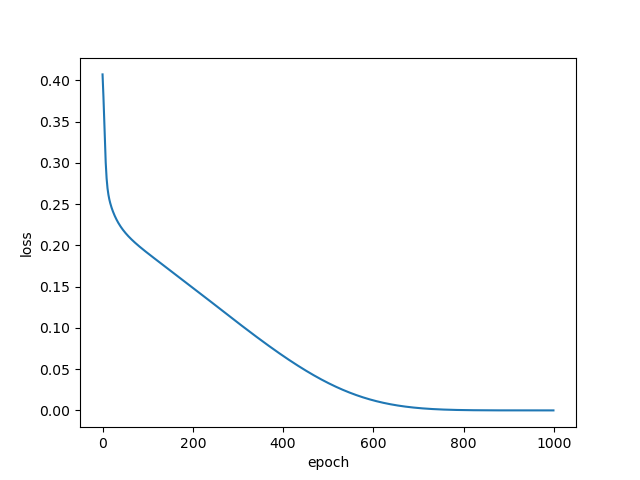
\includegraphics[width=0.5\textwidth]{trivial.png}
  \end{center}
  \caption{Loss function of a basic comparison correction.}
  \label{fig:trivial}
\end{figure}

\begin{minipage}{\textwidth}
We also have found convergence for basic list convergences \ref{fig:list_index} with an incorrect index.
\begin{verbatim}
[index_list_wrong_1
((l : list), (x : int)) -> int
(__index(l, (x + 1)))];

{(index_list_wrong_1({int ; 0, 100, 20, 0, 0, 30, 0}, 1) == 100)};
\end{verbatim}
\end{minipage}
\begin{figure}[h!]
  \begin{center}
    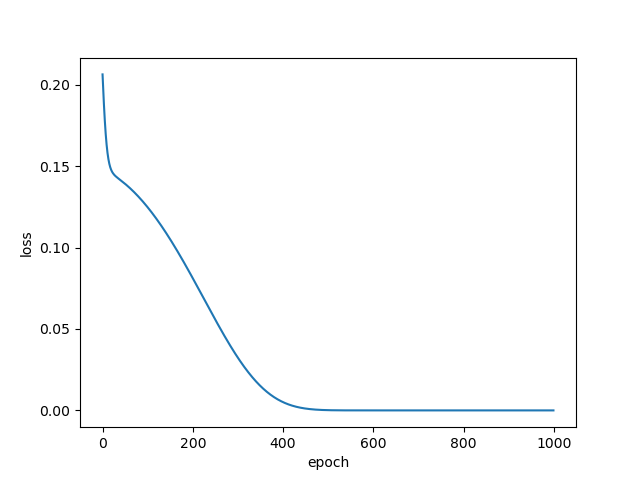
\includegraphics[width=0.5\textwidth]{list_index.png}
  \end{center}
  \caption{Loss function of a basic list index.}
  \label{fig:list_index}
\end{figure}


\begin{minipage}{\textwidth}
A basic for loop that computes $x^3$ also converges to a correct solution with an error in the input of the function \ref{fig:for_loop}.

\begin{verbatim}
[pow3((x : int)) -> int
  (fold [0, 3] (acc, 1) (acc * x))
];

[test_case1() -> bool
  ((pow3(1) == 8))
];

{test_case1()}
\end{verbatim}
\end{minipage}
\begin{figure}[h!]
  \begin{center}
    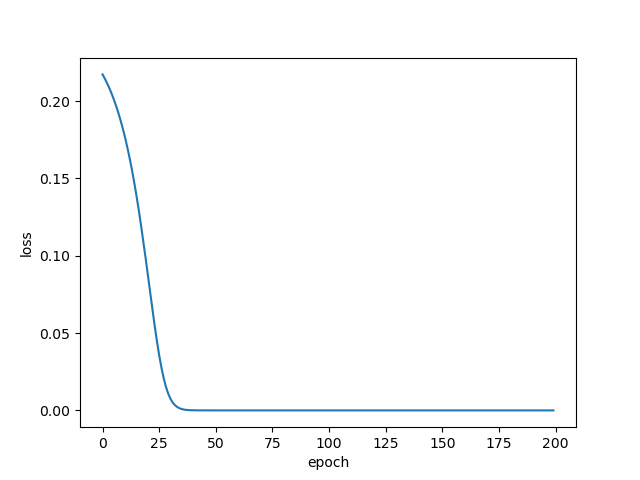
\includegraphics[width=0.5\textwidth]{for_loop.png}
  \end{center}
  \caption{Loss function of a for loop calculating $x^3$.}
  \label{fig:for_loop}
\end{figure}\\\\\\\\\\\\
\begin{minipage}{\textwidth}
The loss function does not always converge. With this implementation of bubble sort with an incorrect index. The convergence of the hyperparameters increases the loss faster than the gradient descent can adjust \ref{fig:bubble_sort}.
\begin{verbatim}
[bubble_sort_pass ((l : list)) -> list
  (fold [0, (__len(l) - 1)] (acc, (l, 0, false))
    ((let curr = __index(0 . acc, 1 . acc)),
      (let next = __index(0 . acc, (1 . acc + 1)))) in
      if (curr > next) then
      (swap(0 . acc, 1 . acc, (1 . acc + 2), next, curr), (1 . acc + 1), true)
      else
      (0 . acc, (1 . acc + 1), 2 . acc))
];

[bubble_sort ((l: list)) -> list
  (while (acc, l) 2 . bubble_sort_pass(acc) 0 . bubble_sort_pass(acc) acc)
];

[swap ((l : list),
       (index_1 : int),
       (index_2 : int),
       (val_1 : int),
       (val_2 : int)) -> list
  (__set_index(__set_index(l, index_1, val_1), index_2, val_2))
];
\end{verbatim}
\end{minipage}
\begin{figure}[h!]
  \begin{center}
    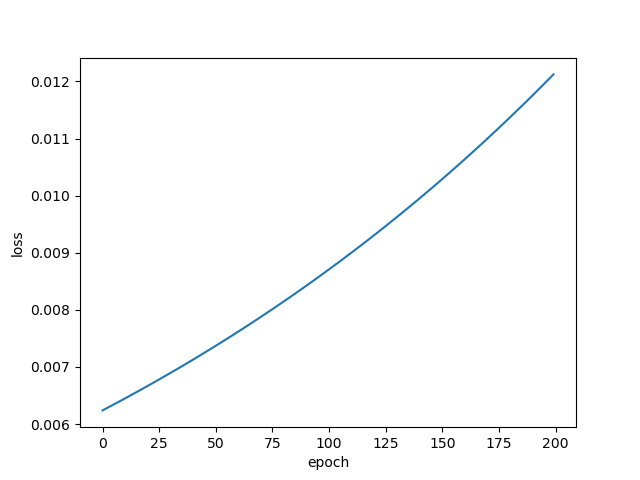
\includegraphics[width=0.5\textwidth]{bubble_sort.png}
  \end{center}
  \caption{Loss function of a bubble sort algorithm, which fails to converge due to the hyperparameters increasing the loss function faster than gradient descent decreasese it.}
  \label{fig:bubble_sort}
\end{figure}
\section{Hessian Newtons Method}
For small programs the number of parameters may be small. We attempted to use a Hessian based machine learning optimization algorithm due to the Hessian being more tractable with its $O(n^2)$ size opposed to gradients $O(n)$ size for small numbers. Opposed to gradient descent below,

\begin{center}
  $W_S := W_S - \lambda \nabla L(W_s)$
\end{center}

, a second order Newtons method will optimize like below.
\begin{center}
  $W_S := W_S - \lambda [H_L(W_s)]^{-1} \nabla L(W_s)$
\end{center}

We gave up on this approach due to the Hessian matrix being non-invertable in many cases. In the case that the gradient of the loss function with respect to any parameters is zero, an entire column and row of the Hessian matrix will be zero, making in non invertable.

\section{Synthetic Data Generation}
We implemented a perturbation of the AST. By adding a small amount of noise to the model parameters, it can introduce incorrect behaviour that can then be given to the model. Elements of $W_S$ can be modified by a gaussian distribution $W_S + N(0, I)$. This method can allow testing the accuraccy of the model at correcting programs, and finidng cases where it is unable to.

\section{Limitations}
\subsection*{While loops}
While loops are slow. Because it uses an algebreic handler, each iteration of a while loop requires runing the entire rest of the program. This method can result in a runtime complexity of up to $O(k^n)$ where $n$ is the number of while loops.

Another problem is the innaccuracy of while loops. The program below calculates $2^x$, and each iteration of the while loop doubles in size.
\begin{verbatim}
[exp2((x : int)) -> int
  (while (acc, (0, 1)) __not((0 . acc == x)) ((0 . acc + 1), (1 . acc * 2)) 1 . acc)
];
\end{verbatim}
A problem ariseses when the contribution of a while loop grows faster than the conditional decreases each iteration's contribution. This effect heavily biases the while loop towards later iterations, and our framework is unable to correct this program.

\section{Conclusion and Future Work}
This work demonstrates a proof-of-concept for automatically correcting program errors using deep learning optimization methods.

Future work can include:
\begin{itemize}
\item \textbf{Performance Optimization:} We ported the parts of the framework to Cuda, but did not result in significant speedup. We belive this to be the lack of large tensor operations, because our model doesn't necessarilly have feed forward networks. We believe speedup can still be achieved with cuda graph computations which can partially compile the computational graph of an instantiation of our model. A multithreaded approch to while loops iterations which are trivially parralelizable, could also be implemented.
\item \textbf{Hyperparameter Adjustment:} We require more expirementation for different dynamic hyperparameter adjustment. Current exponential decay fails for many of the more complex programs.
\item \textbf{Comprehensive Evaluation:} We require testing on non-trivial codebases to assess practical utility at a larger scale.
\end{itemize}

\bibliographystyle{abbrv}
\bibliography{refs}
\end{document}
\documentclass{article}
